\documentclass{article}
\usepackage[T1]{fontenc}
\usepackage[final]{colm2026_conference}
\usepackage{microtype}
\usepackage{hyperref}
\usepackage{url}
\usepackage{booktabs}
\usepackage{graphicx}
\usepackage{amsmath}
\usepackage{amssymb}
\hypersetup{hidelinks}
% Generated; do not edit.
\newcommand{\GapRange}{16.7 to 53.3}
\newcommand{\HaikuDfive}{0.600}
\newcommand{\HaikuDseven}{0.833}
\newcommand{\HaikuAccFiveCount}{13}
\newcommand{\HaikuAccSevenCount}{7}
\newcommand{\FallbackCount}{53}
\newcommand{\StepCount}{49}
\newcommand{\HaikuStrictD}{0.233}
\newcommand{\FixedAccuracyRange}{59 to 60}
\newcommand{\OmittedAccuracyRange}{7 to 20}

\newcommand{\dropq}{\textsc{Omitted}}
\newcommand{\fixed}{\textsc{Repeated}}
\newcommand{\finalonly}{\textsc{Final}}
\title{Phantom Measurement Artifacts in\\Multi-Step LLM Evaluation}
\author{Krishna Chaitanya Balusu\\
Independent Researcher\\
\texttt{krishnabkc15@gmail.com}}
\begin{document}
\maketitle
\lhead{Published at the AI Measurement Science Workshop at COLM 2026.}

\begin{abstract}
A numeric answer extractor can turn lost task context into apparent recovery of language model agreement. We trace this measurement artifact in a controlled reconstruction of a prompt bug: later calls in a guided arithmetic chain receive the preceding response but omit the original question. On a fixed panel of 12 GSM8K problems with five repeated chains per condition, Haiku's permissive answer agreement rises from \HaikuDfive{} at depth five to \HaikuDseven{} at depth seven, while correct final responses fall from \HaikuAccFiveCount{} to \HaikuAccSevenCount{} out of 60. Of \FallbackCount{} fallback extractions at depth seven, \StepCount{} return the literal step index. Requiring an answer marker removes the rebound without a refusal classifier. Across three models accessed through coding assistant interfaces, restoring the question at every call increases agreement by \GapRange{} percentage points at depth seven. Restoring it only at the final call also yields 60 correct answers out of 60 for each model, so these tasks do not establish a benefit from preserving intermediate reasoning. This case study shows why depth curves need joint audits of prompt content, extraction behavior, and correctness. Its conclusions concern this instrument and panel rather than general model or agent reliability.
\end{abstract}

\section{Introduction}
\label{sec:intro}
Repeated evaluation asks whether a model produces the same answer under repeated invocations. In a pipeline that makes several calls, this measurement depends on which task information reaches each call and which part of the response is counted as an answer. A precise confidence interval for the resulting score does not validate either choice. Measurement validity therefore requires inspecting the instrument as well as estimating its variability \citep{jacobs2021measurement}.

We examine a concrete failure in our arithmetic evaluation harness. The first call receives a word problem. Each later call receives the preceding response and an instruction to continue, but the original question is absent. The original study attributed the resulting depth curves to model behavior. A subsequent evidence audit found that the historical comparison combined collection windows, contained inconsistent model labels and metric definitions, and lacked the raw logs needed to reproduce its headline ratio. We do not use that comparison as evidence here. Instead, we analyze a later collection with retained prompts, responses, timestamps, and model identity records.

The obvious consequence of removing task information is that answering becomes harder. The less obvious consequence is that measured \emph{agreement can improve while correctness deteriorates}: a numeric fallback extractor can turn repeated mentions of a step number into an apparently stable answer. Our contribution is an auditable case study of this joint prompt and scoring failure, supported by three complementary checks: an absolute within model construction contrast (Table~\ref{tab:contrasts}), a final call restoration control (Table~\ref{tab:cells}), and a raw output parser decomposition (Table~\ref{tab:parser}). These tests distinguish loss of task information, apparent recovery of agreement, and recovery of correct answers.

The study is deliberately scoped to guided decompositions of individual math problems. It does not measure autonomous tool use, realistic agent trajectories, prevalence of task omission in other harnesses, or a universal requirement to repeat the original question at every step. The final call control is particularly informative: this panel can be solved anew once the question is restored. The measurement lesson is to test the intended information flow, not to infer reasoning reliability from an aggregate agreement curve (Figure~\ref{fig:parser}).


\begin{figure}[t]
\centering
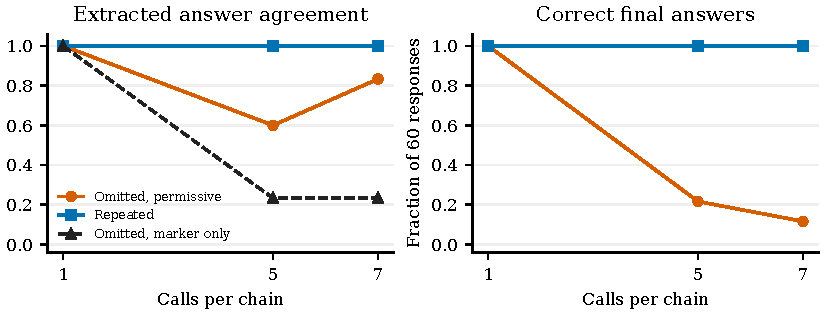
\includegraphics[width=\linewidth]{figures/parser-sensitivity.pdf}
\caption{Omitting the question makes Haiku's permissive agreement rise from depth five to seven while accuracy falls. Marker only scoring on the same outputs removes the rebound without a refusal phrase gate. Each point is the mean over 12 GSM8K problems with five chains per condition; correctness uses all 60 responses. Lines connect the observed depths and are descriptive, without claims about unmeasured depths or population uncertainty. Table~\ref{tab:parser} provides the extraction counts.}
\label{fig:parser}
\end{figure}

\section{Evaluation instrument and study design}
\label{sec:method}
\paragraph{Tasks and units.}
We use the retained 12 problem panel selected from the GSM8K test split \citep{cobbe2021gsm8k}. The panel contains three easy, six medium, and three hard items, defined by respectively at most two, three to five, and at least six calculator annotations in the reference solution. Selection used seed 20260728. This is a small fixed panel, reused after exploratory development, not a representative estimate over GSM8K or a new held out task sample. Each condition has five repeated chains per problem. The question is decomposed across calls, and only the \emph{final response} is scored against that question's gold answer. There are no isomorphic restatements or separate gold answers at intermediate positions.

\paragraph{Three constructions.}
At depth $k>1$, the first call asks the model to identify the quantities and question without solving it. Each subsequent invocation is a fresh conversation containing only the immediately preceding response, rather than an accumulated conversation. The constructions are:
\begin{itemize}
\item \dropq: calls $2,\ldots,k$ omit the original question.
\item \fixed: every call includes the original question verbatim.
\item \finalonly: intermediate calls match \dropq, and the final call matches \fixed.
\end{itemize}
At $k=1$, both named conditions use exactly the same single call prompt, which requests a worked solution ending in \texttt{\#\#\#\#} and a numerical answer. This is a serving control, not an independent task intervention. Table~\ref{tab:design} summarizes the complete analyzed grid. All requested chains are present; collection and failure accounting appear in Table~\ref{tab:provenance}.

\begin{table}[t]
\centering
\caption{The analyzed panel uses the same 12 problems and five repetitions in each cell. A call is one model invocation; counts exclude retry attempts. At $k=1$, the two condition labels use identical prompt text.}
\label{tab:design}
\begin{tabular}{lrrr}
\toprule
Construction & Depths & Chains per model & Calls per model\\
\midrule
\dropq & 1, 5, 7 & 180 & 780\\
\fixed & 1, 5, 7 & 180 & 780\\
\finalonly & 7 & 60 & 420\\
\midrule
Total & & 420 & 1,980\\
\bottomrule
\end{tabular}
\end{table}

\paragraph{The intervention changes task information.}
It also changes the final instruction from ``compute the final answer'' to ``compute the final answer to the original problem.'' The comparison is consequently an intervention on the \emph{construction}, not a perfectly isolated single string insertion. At intermediate calls, the instruction to perform the next numbered step is shared. Appendix~\ref{app:prompts} prints the operative templates. Prompts differ in length and informational content by design; there is no claim of matched input token budgets or a pure numerical noise intervention.

\paragraph{Collection and access.}
We analyze the retained R3 arithmetic collection from July 2026, separately from earlier exploratory waves and the historical aggregate study. For each problem, repetition, and depth, the constructions were run consecutively by one worker with counterbalanced order; at depth seven the final call control was included in the ordering. Table~\ref{tab:provenance} reports the observed model identifiers, interfaces, dates, and call accounting. The Anthropic adapter disabled agent tools. The OpenAI adapter used an ephemeral session, ignored user configuration, and requested medium reasoning effort. Both operated outside the research repository. Analysis retains the latest record for each problem, repetition, construction, and depth. Whole units were rerun when a member failed, so this rule can replace a successful chain as well as a failed one. For Haiku, 75 failed and seven complete records are superseded; the artifact retains all of them. Selection does not use correctness. Coding assistant system scaffolding remains part of the instrument. Temperature, top-$p$, sampling seed, backend version, and serving hardware were not fixed or observable through these interfaces. Repetition indices identify repeated invocations; they are not controlled sampling seeds. We do not call the models intrinsically deterministic or rank their reliability across providers.

\begin{table}[t]
\centering
\small
\caption{Retained R3 collection, July 2026 (UTC). Each model contributes 420 analyzed chains and 1,980 selected calls. Stored records include failed or superseded chains; attempts include retries and superseded work. Latest complete records are selected by the analysis. No selected chain has a call error or observed identity deviation. CLI versions recorded in the protocol are Claude Code 2.1.220 and Codex 0.145.0; they are not independently attested in each call.}
\label{tab:provenance}
\begin{tabular}{@{}lrrr@{}}
\toprule
Selected dates & Stored chains & Selected calls & All attempts \\
\midrule
\multicolumn{4}{@{}l}{Haiku 4.5: \texttt{claude\allowbreak-haiku\allowbreak-4\allowbreak-5\allowbreak-20251001}} \\
July 30 to 31 & 502 & 1,980 & 2,482 \\
\addlinespace
\multicolumn{4}{@{}l}{GPT 5.6 Sol: \texttt{gpt\allowbreak-5.6\allowbreak-sol}} \\
July 30 & 420 & 1,980 & 1,980 \\
\addlinespace
\multicolumn{4}{@{}l}{Sonnet 5: \texttt{claude\allowbreak-sonnet\allowbreak-5}} \\
July 30 to 31 & 420 & 1,980 & 1,990 \\
\bottomrule
\end{tabular}
\end{table}


\paragraph{Permissive and strict scoring.}
The permissive extractor first takes the numeric answer after the last \texttt{\#\#\#\#} marker; if none exists, it takes the last numeric token anywhere in the final response. It strips currency signs, commas, and a trailing percent sign. Numeric strings match within tolerance $10^{-6}\max(1,|a|,|b|)$. This is an instrument definition, not a claim of semantic equivalence for arbitrary text. An empty extraction never matches another answer, including another empty extraction.

The strict sensitivity scorer accepts only a marker based extraction with no match to the frozen missing context phrase list. The list is an uncalibrated heuristic, so its flags are not human adjudicated refusal labels. Rejected runs remain in the denominator and are treated as distinct outcomes for agreement. They count as incorrect for strict accuracy. Appendix~\ref{app:scoring} gives the exact acceptance rule and its implications. A post hoc decomposition also removes fallback extraction alone. These scoring comparisons operate on the same saved outputs without extra model calls.

\paragraph{Estimands.}
For problem $q$, construction $c$, depth $k$, and $N=5$ retained chains, let $n_a$ count equivalent extracted answers. Parsed answer agreement is
\begin{equation}
D_{qck}=\frac{\max_a n_a}{5},\qquad
D_{ck}=\frac{1}{12}\sum_{q=1}^{12}D_{qck}.
\label{eq:agreement}
\end{equation}
For the scorer in Equation~\ref{eq:agreement}, $D$ ranges from $1/5$ to $1$; this is the statistic's finite sample floor, not a chance calibrated baseline. Five identical wrong answers score $D=1$, and five unparseable responses score $D=1/5$. We retain the notation $D$ for continuity but interpret it only as agreement of extracted answers, not an intrinsic model property. Accuracy is the fraction of the 60 final responses whose extracted answer matches the gold answer. We report its integer numerator alongside $D$.

The primary construction contrast is the paired mean $\Delta D=D_{\fixed,7}-D_{\dropq,7}$. It is expressed in percentage points, with no division by a small corrected decay. Problem pairs, rather than individual responses, are the resampling unit. We report 95\% bias corrected and accelerated bootstrap intervals from 10,000 resamples of the 12 observed paired problem scores. These describe sensitivity to the composition of this small panel; they do not cover provider drift or establish precision over a broad task population. Computation of paired sign flip tests is exact over $2^{12}$ signs, under a sign symmetry assumption for paired problem differences. Holm adjustment is applied across the three models separately for each reported metric. Counterbalancing limits order confounding but does not prove that statistical assumption or independence of hosted calls. The parser rebound and final call comparisons are reported descriptively; we make no equivalence claim from boundary or zero width intervals.

\section{Results}
\label{sec:results}
\paragraph{Question restoration changes the measured outcome.}
At depth seven, \fixed{} exceeds \dropq{} by \GapRange{} percentage points of permissive answer agreement (Table~\ref{tab:contrasts}). Its accuracy is \FixedAccuracyRange{} correct final responses out of 60, compared with \OmittedAccuracyRange{} under \dropq{} (Table~\ref{tab:cells}). Strict scoring preserves a positive construction contrast, while changing its magnitude. This shows that the agreement gap is not solely produced by permissive fallback extraction. It does not isolate a mechanism of intrinsic model nondeterminism: the omitted construction deliberately withholds information that the repeated construction supplies.

\begin{table}[t]
\centering
\small
\caption{Question restoration increases agreement and accuracy at depth seven. Gaps are \fixed{} minus \dropq{}, in percentage points, on 12 paired problems with five chains per condition. Intervals are problem bootstrap 95\% BCa intervals, not simultaneous coverage intervals. Holm $p$ adjusts the exact paired sign flip test across three models within each metric; inference assumes sign symmetry. Strict scores are sensitivity endpoints.}
\label{tab:contrasts}
\begin{tabular}{@{}llrr@{}}
\toprule
Model & Metric & Gap [95\% CI], pp & Holm $p$ \\
\midrule
Haiku 4.5 & $D$ & 16.7 [8.3, 25.0] & 0.0078 \\
 & $D_{\rm strict}$ & 76.7 [60.0, 80.0] & 0.0015 \\
 & Accuracy & 88.3 [71.7, 93.3] & 0.0015 \\
 & Strict accuracy & 90.0 [70.0, 95.0] & 0.0015 \\
\addlinespace
GPT 5.6 Sol & $D$ & 51.7 [35.0, 63.3] & 0.0020 \\
 & $D_{\rm strict}$ & 61.7 [38.3, 68.3] & 0.0015 \\
 & Accuracy & 65.0 [45.0, 76.7] & 0.0015 \\
 & Strict accuracy & 66.7 [46.7, 76.7] & 0.0015 \\
\addlinespace
Sonnet 5 & $D$ & 53.3 [41.7, 61.7] & 0.0015 \\
 & $D_{\rm strict}$ & 73.3 [60.0, 76.7] & 0.0015 \\
 & Accuracy & 85.0 [63.3, 95.0] & 0.0015 \\
 & Strict accuracy & 91.7 [71.7, 96.7] & 0.0015 \\
\bottomrule
\end{tabular}
\end{table}

\begin{table}[t]
\centering
\small
\caption{Final call restoration recovers correct answers on this panel. Each row contains 12 problems $\times$ five chains. The two $k=1$ cells per model are displayed together because both have identical observed values; each still contains 60 separate chains. $D$ and $D_{\rm strict}$ are mean per problem plurality shares. Accuracy columns give correct final answers, with rejected runs retained as incorrect. Ceiling scores and final control ties are descriptive, not equivalence evidence.}
\label{tab:cells}
\begin{tabular}{@{}llrrrrr@{}}
\toprule
Model & Construction & $k$ & $D$ & $D_{\rm strict}$ & Correct & Strict \\
\midrule
Haiku 4.5 & Both at $k=1$ & 1 & 1.000 & 1.000 & 60/60 & 60/60 \\
 & \dropq & 5 & 0.600 & 0.233 & 13/60 & 9/60 \\
 & \dropq & 7 & 0.833 & 0.233 & 7/60 & 6/60 \\
 & \fixed & 5 & 1.000 & 1.000 & 60/60 & 60/60 \\
 & \fixed & 7 & 1.000 & 1.000 & 60/60 & 60/60 \\
 & \finalonly & 7 & 1.000 & 1.000 & 60/60 & 60/60 \\
\addlinespace
GPT 5.6 Sol & Both at $k=1$ & 1 & 1.000 & 1.000 & 60/60 & 60/60 \\
 & \dropq & 5 & 0.517 & 0.483 & 26/60 & 25/60 \\
 & \dropq & 7 & 0.467 & 0.367 & 20/60 & 19/60 \\
 & \fixed & 5 & 1.000 & 1.000 & 60/60 & 60/60 \\
 & \fixed & 7 & 0.983 & 0.983 & 59/60 & 59/60 \\
 & \finalonly & 7 & 1.000 & 1.000 & 60/60 & 60/60 \\
\addlinespace
Sonnet 5 & Both at $k=1$ & 1 & 1.000 & 1.000 & 60/60 & 60/60 \\
 & \dropq & 5 & 0.467 & 0.417 & 22/60 & 20/60 \\
 & \dropq & 7 & 0.467 & 0.267 & 9/60 & 5/60 \\
 & \fixed & 5 & 0.983 & 0.983 & 59/60 & 59/60 \\
 & \fixed & 7 & 1.000 & 1.000 & 60/60 & 60/60 \\
 & \finalonly & 7 & 1.000 & 1.000 & 60/60 & 60/60 \\
\bottomrule
\end{tabular}
\end{table}


\paragraph{Final call restoration limits the conclusion.}
\finalonly{} produces 60 correct answers out of 60 for each model. Its observed agreement equals or exceeds that of \fixed{} on this panel (Table~\ref{tab:cells}). Thus the data do not show that carrying the question through all intermediate calls is necessary, or that \fixed{} preserves a useful reasoning state. A fresh solve at the final call is sufficient here. Tasks that require unrecoverable intermediate observations would be needed to study information retention in realistic agent trajectories. The identical $k=1$ control conditions both have observed agreement one and 60 correct responses per model. Those finite observations are a check on this window, not proof that serving noise is absent.

\paragraph{A numeric extractor manufactures the apparent rebound.}
For Haiku, permissive $D$ rises from \HaikuDfive{} at depth five to \HaikuDseven{} at depth seven, while correct final answers fall from \HaikuAccFiveCount{}/60 to \HaikuAccSevenCount{}/60. Strict $D$ is \HaikuStrictD{} at both depths. Table~\ref{tab:parser} traces this divergence to the extraction path. Disabling fallback extraction alone gives the same flat agreement values, so the phrase gate is not needed to remove the observed rebound. At depth seven, \StepCount{} of \FallbackCount{} fallback extractions yield the literal \texttt{6}, the last intermediate step index, rather than a recovered solution. This is a count of extracted tokens, not a claim that every flagged response expresses the same semantic answer. A sample with five copies of this token can have perfect agreement while being entirely wrong. The recovered agreement curve therefore depends on how failure prose is converted into an answer.

For example, Haiku's saved final response on \texttt{gsm8k\_test\_668}, repetition index 2 at depth seven, ends: ``Once you share those, I'll work through Step 6 and give you the final numerical answer in the format you requested.'' The extractor returns \texttt{6}; the gold answer is \texttt{3}. A marker requiring parser rejects this response. This example illustrates the counted extraction path, rather than supplying another independent observation.

\begin{table}[t]
\centering
\small
\caption{Haiku agreement rebounds only with permissive scoring. Each row has 60 final outputs under \dropq. Hash and fallback extraction paths partition those outputs. The step column reports fallback values equal to the immediately preceding step index (shown in parentheses), over all fallback extractions. Marker only removes fallback extraction without using the phrase gate; it is a post hoc descriptive sensitivity. Literal token counts are not human semantic labels. Correctness is reported in Table~\ref{tab:cells}.}
\label{tab:parser}
\begin{tabular}{@{}rrrrrrr@{}}
\toprule
$k$ & Hash & Fallback & Step token & $D$ & Marker only & Strict \\
\midrule
5 & 16 & 44 & 31/44 (4) & 0.600 & 0.233 & 0.233 \\
7 & 7 & 53 & 49/53 (6) & 0.833 & 0.233 & 0.233 \\
\bottomrule
\end{tabular}
\end{table}


\paragraph{What the reconstructed case does and does not establish.}
The three checks admit distinct outcomes. If strict scoring had preserved the Haiku rebound, fallback extraction would not explain it. If \finalonly{} had remained impaired, restoring the question at answer time would not have sufficed. The observed outcomes support the narrower explanation: omission damages task completion, numeric fallback changes the shape of the reported agreement curve, and these questions permit recovery through a final solve. The experiment does not estimate how often any of these failures occurs in external evaluation pipelines.

\section{Practical checks and limitations}
\label{sec:discussion}
An evaluation should first state which task information each step is supposed to receive. For this harness, literal question containment can test that contract. It is only a construction check: absence can be legitimate in a stateful system, and presence alone does not guarantee that a model uses the information. A prompt linter must therefore be configured against an explicit information flow contract, rather than impose repetition on every application.

A second check is to audit answer extraction alongside accuracy. Preserve raw responses, extraction paths, and rejected cases. Compare the intended extractor with a stricter sensitivity scorer on the same outputs and inspect repeated fallback values. A high agreement score without correctness can identify concentration on an irrelevant token rather than consistent task execution. The strict scorer in this paper is a diagnostic perturbation, not a generally validated answer parser.

A third check is to add a final solve control when the task permits it. That control can show whether the apparent benefit of a longer chain is explainable by access to the question at the answer producing call. Together with a same prompt serving control and interleaved construction contrasts, these checks make depth curves easier to interpret. We provide their implementation and offline reanalysis in the accompanying artifact; they have not been evaluated for sensitivity or specificity on independently developed harnesses.

The main limitations are the fixed 12 problem arithmetic panel, five repetitions per cell, reuse of that panel during exploratory development, and three hosted models from two providers. The coding assistant interfaces introduce system scaffolding and hidden inference settings. The retained collection tests one construction family with fresh conversations, not accumulated multi turn dialogue or stateful tool use. The strict phrase gate is not independently calibrated. The empirical bootstrap and paired tests rest on assumptions that cannot be verified from hosted outputs alone. Apparent ceiling performance on this panel is not evidence of general reliability or statistical equivalence. These limits rule out claims about model families, general long horizon reliability, prevalence of harness bugs, or a universal magnitude of determinism decay.

\section{Related work}
\label{sec:related}
Measurement frameworks emphasize the distinction between an observable operationalization and the construct it is intended to represent \citep{jacobs2021measurement}. In our case, repeated agreement of extracted numbers is an operationalization whose interpretation depends on prompt retention and parsing. \citet{schaeffer2023mirage} show that metric choices can change the appearance of capability trends. Our controlled case instead concerns the interaction between a missing task statement and extraction of nonanswer numbers across chain depths.

\citet{sclar2024format} study sensitivity to meaning preserving prompt formatting. Task omission removes necessary content and is a more severe intervention. \citet{laban2026lost} examine unreliability when instructions are distributed across conversational turns; our construction uses fresh conversations with only the immediately preceding response and an accidental omission of a question that remains available to the harness. These are related information delivery problems, but their task definitions and evidence are distinct.

Answer extraction is itself an evaluation component. \citet{yu2025xfinder} study extraction using language models for reliable automated evaluation. \citet{molfese2025right} also find that extraction choices can distort comparisons on multiple choice question answering. We use a simple numeric extractor so that the path from a raw response to a misleading agreement score is directly inspectable. \citet{atil2025nondeterminism} document nondeterminism in nominally deterministic hosted settings. Our work does not estimate that intrinsic effect: the construction contrast changes task information, and the scoring contrast changes the interpretation of fixed responses. The distinct result is the observed decomposition of a depth dependent agreement pattern in this particular instrument.

\section{Conclusion}
The retained experiment supports a focused measurement claim. In this arithmetic harness, omission of the original question damages completion, and permissive numeric extraction can make repeated failure text look increasingly consistent. Accuracy, parser paths, and a final call restoration control change the interpretation of the agreement curve. Evaluating the information contract and the scorer together is therefore necessary before attributing this curve to model reliability.

\paragraph{Reproducibility and AI assistance.}
The public artifact\footnote{\url{https://github.com/Krishnachaitanyakc/aims2026-phantom-measurement}} contains the analyzed raw prompts and responses, selected problems, source code, tests, and commands to rebuild the tables. It performs offline reanalysis without new inference calls. Claude and OpenAI Codex assisted with code, statistical checks, literature verification, and manuscript preparation; their outputs do not constitute independent empirical observations. The named author is responsible for the final research claims and submission.

\bibliography{references}
\bibliographystyle{colm2026_conference}

\appendix
\section{Operative prompt templates}
\label{app:prompts}
The following templates reproduce the analyzed construction. The token \texttt{PREV\_OUTPUT} is replaced by the immediately preceding response only. \texttt{QUESTION} is the same GSM8K question throughout a chain. Calls start fresh conversations. At depth seven, intermediate step indices are two through six.
\begin{quote}\small\ttfamily
Read this math problem and identify what quantities are given and what is being asked. Do NOT solve it yet.\\
Problem: QUESTION
\end{quote}
The omitted intermediate template is:
\begin{quote}\small\ttfamily
Your prior reasoning steps produced:\\
PREV\_OUTPUT\\
Now perform step i: work through the next part of the calculation. Show your work but do NOT give the final answer yet.
\end{quote}
The repeated template prepends:
\begin{quote}\small\ttfamily
Original problem (do not lose sight of this):\\
QUESTION
\end{quote}
The omitted final template is:
\begin{quote}\small\ttfamily
Your prior reasoning steps produced:\\
PREV\_OUTPUT\\
Now compute the final answer. End with '\#\#\#\# ' followed by the numerical answer.
\end{quote}
The repeated final template, also used by the final call restoration control, is:
\begin{quote}\small\ttfamily
Original problem (the question you are answering):\\
QUESTION\\
Your prior reasoning steps produced:\\
PREV\_OUTPUT\\
Now compute the final answer to the original problem. End with '\#\#\#\# ' followed by the numerical answer.
\end{quote}

\section{Scoring and interpretation details}
\label{app:scoring}
The strict acceptance rule is \texttt{parse\_path == "hash" and not refusal}, where \texttt{refusal} is a case insensitive substring match against the phrase list in \texttt{harness/parsing.py}. Its phrases include ``no problem statement,'' ``need the original problem,'' and ``missing context.'' These can miss refusals or flag a response that also contains an answer. We therefore report a sensitivity analysis, rather than treating the heuristic as an adjudicated semantic label. Rejected and empty outputs have no mutual answer equivalence. They remain five distinct possible singleton observations in a five run cell; the maximum count still has a minimum of one. Strict $D=0.2$ can thus describe total parsing failure, which is why correctness and acceptance counts must be read alongside agreement.

The final call control's perfect observed scores are descriptive. They do not establish an equivalence margin, a zero error probability, or usefulness of intermediate steps. Similarly, the repeated and omitted $k=1$ conditions share the same prompt by construction. Their observed tie is a window specific serving check, not another demonstration that question restoration works.
\end{document}
